The conceptual architecture introduced in the previous chapter provides the theoretical foundation for transforming unstructured speech into structured templates. This chapter shifts focus from design to realization, demonstrating how the multi-agent pipeline was implemented in practice. The implementation details cover technology selection, system workflow, concrete agent implementations, and the realization of the four architectural strategies. Finally, challenges and key design decisions encountered during development are discussed.

\section{Technology Stack and Rationale}
\label{sec:tech-stack}

The implementation of the \textit{Invox} system employs a modular monolith architecture that balances development simplicity with operational flexibility. The core application executes as a single Node.js service containing all five agents, while specialized components such as vector search and embedding generation operate as external services. This hybrid approach preserves the benefits of modular design while avoiding the operational complexity typically associated with fully distributed microservice deployments \cite{fowler2015monolith,microservices_newman}.

\subsection*{Architecture Pattern: Modular Monolith with External Services}

The system follows a modular monolith pattern in which all agents (STT, RAG, IE, CF, VER) are implemented as cohesive modules within a single Node.js application. This design choice offers several advantages: a unified codebase that reduces coordination overhead, simplified debugging, and consistent versioning across agents. In-process inter-agent communication minimizes latency compared to network-based microservices, while modularity is maintained through well-defined interfaces that preserve separation of concerns.

External specialized services are integrated via network calls. \textbf{OpenSearch} provides vector similarity search, accessible through \texttt{http://opensearch:9200}; a dedicated embedding service generates dense vector representations; and external LLM APIs (OpenAI, Google) handle model inference. This hybrid approach leverages specialized infrastructure where necessary, while retaining the core template-filling logic within a unified application \cite{opensearch_knn}.

\subsection*{Containerization and Deployment}

The entire system is containerized using \textbf{Docker}. The main application runs in a single container, ensuring a consistent runtime environment across development and production. Containerization simplifies dependency management, enables horizontal scaling through replication, and facilitates seamless integration with external services. \textbf{Docker Compose} orchestrates the multi-service deployment, coordinating the main application container alongside OpenSearch and other dependencies \cite{docker_docs}.

\subsection*{Backend Implementation}

The backend is implemented in \textbf{Node.js} with \textbf{Express}, providing a robust foundation for the agent pipeline. The system employs the \textbf{Vercel AI SDK} to realize a plugin-like architecture for LLM integration. This abstraction enables seamless switching between AI providers (OpenAI, Google, Anthropic), simplifies the addition of new models with minimal code changes, and future-proofs the system against the rapid evolution of the AI ecosystem \cite{llm_orchestration_survey}. Type-safe communication between frontend and backend is achieved through \textbf{tRPC}, while \textbf{JSON} serves as a flexible exchange format for inter-agent communication.

\subsection*{External Service Integration}

\textbf{OpenSearch} functions as the vector database for the RAG agent, enabling efficient semantic search over historical templates. A dedicated embedding generation service produces dense vector representations, which underpin similarity matching. Both services expose \textbf{REST APIs}, maintaining clear service boundaries while enabling specialized functionality \cite{opensearch_knn}.

\subsection*{Frontend Interface}

The user interface is implemented in \textbf{React}, selected for its component-based architecture that aligns naturally with the modular design of the template-filling system. React's virtual DOM and state management capabilities enable efficient rendering of dynamic content, such as structured templates and extracted fields with confidence indicators.

To ensure modern and accessible UI design, the system integrates the \textbf{shadcn/ui} component library. This provides reusable, consistent components with built-in design principles, thereby reducing frontend development overhead while ensuring a professional user experience for template review and correction workflows.

\subsection*{Data Persistence and Retrieval}

Persistent storage is provided by \textbf{PostgreSQL}, a relational database well-suited for structured data with complex relationships. The MUC-4 template schema maps naturally onto relational structures: fields such as incident type, date, and location are represented as structured columns, while more flexible attributes are stored in \texttt{JSONB} to allow schema evolution \cite{postgresql_jsonb}.

The \textbf{Sequelize} ORM is employed for schema definition, object mapping, secure query generation, and migration management. For vector similarity search, \textbf{OpenSearch} with the \texttt{knn} plugin enables efficient retrieval of relevant historical templates using dense embeddings \cite{opensearch_knn}.

\subsection*{Authentication and Security}

Authentication and role-based access control are managed via \textbf{Keycloak}, an open-source identity and access management solution supporting OAuth2 and OpenID Connect \cite{rfc6749,openid_connect}. Keycloak ensures secure integration with backend services and allows fine-grained role assignments—essential for collaborative workflows in which different users require distinct levels of access to system functionality.

\subsection*{Architecture Rationale}

The modular monolith pattern was chosen as a pragmatic balance between simplicity and flexibility. It combines the development velocity of a monolith with the architectural clarity of modular design \cite{fowler2015monolith}. The plugin-oriented LLM integration enabled by the Vercel AI SDK ensures adaptability to new models and capabilities as the field evolves, while containerized deployment guarantees reliable operation at scale. This architecture thereby provides a future-proof, maintainable, and efficient foundation for the \textit{Invox} system.

\section{System Workflow}
\label{sec:system-workflow}

This section describes the operational workflow of the Invox system, tracing the transformation of unstructured input into verified structured templates. The workflow implements the conceptual pipeline from Chapter~\ref{chap:concept} through a sequence of processing stages with user-driven quality control.

\subsection*{End-to-End Processing Flow}

The system workflow begins with user input and proceeds through six sequential stages:

\begin{enumerate}
    \item \textbf{Input Reception}: Users provide input through speech (audio recording) or direct text entry via the web interface. The system accepts both modalities and routes them appropriately through the processing pipeline.
    
    \item \textbf{Speech Recognition}: For audio inputs, the system invokes the Whisper ASR service to generate transcripts with confidence scores and timestamps. Text inputs proceed directly to the next stage.
    
    \item \textbf{Context Retrieval}: The RAG agent queries the vector database to retrieve the most relevant historical templates and examples, providing contextual guidance for the extraction process.
    
    \item \textbf{Information Extraction}: Based on the selected strategy (S1–S4), the system processes the input:
    \begin{itemize}
        \item \textbf{S1 (Single LLM)}: A single language model extracts all template fields in one pass
        \item \textbf{S2 (Slot-wise)}: Multiple LLM calls extract each field independently  
        \item \textbf{S3/S4 (Multi-LLM)}: Multiple models generate candidate answers, with a dedicated judge LLM selecting the optimal response through comparative analysis
    \end{itemize}
    
    \item \textbf{Consistency Enforcement}: The CF agent normalizes dates to ISO format, standardizes entity names, and enforces schema compliance through deterministic transformation rules.
    
    \item \textbf{Quality Assessment and Presentation}: The system assigns confidence scores to each extracted field and presents the complete template to the user for review and potential correction.
\end{enumerate}

\subsection*{User-Driven Quality Control}

The system employs a user-in-the-loop approach where quality assurance is primarily driven by human judgment:

\textbf{Confidence-Based Presentation}: Fields with lower confidence scores are visually highlighted, directing user attention to potentially problematic extractions.

\textbf{Multi-Model Decision Making}: In strategies S3 and S4, the judge LLM evaluates candidate answers from multiple models, selecting the most appropriate response based on coherence, accuracy, and alignment with the input context.

\textbf{User-Initiated Reprocessing}: If users are unsatisfied with results, they can modify their input and resubmit for reprocessing, creating an iterative refinement cycle driven by human assessment rather than automated detection.

\subsection*{Knowledge Accumulation}

Successfully processed templates are indexed in the vector database, enabling the RAG agent to leverage an expanding knowledge base for improved context retrieval in future processing cycles.
\section{Agent Implementation}
\label{sec:impl-agents}

This section details the concrete implementation of each agent in the Invox system, covering their API contracts, processing logic, and integration patterns. Each agent exposes well-defined TypeScript interfaces and follows consistent error handling patterns. The implementation is designed to be domain-agnostic, supporting arbitrary template schemas across healthcare, manufacturing, administrative, and other domains.

\subsection{Speech-to-Text (STT) Agent}
\label{subsec:impl-stt}

The STT agent provides a single entry point \texttt{transcribeForm} that converts audio inputs to structured transcripts using OpenAI's Whisper model.

\textbf{API Contract:}
\begin{verbatim}
interface TranscribeInput {
  file: {
    base64: string;         // Base64-encoded audio data
    mimetype: string;       // "audio/wav" | "audio/mpeg" | "audio/m4a"
    originalname: string;
  };
}

interface TranscribeResponse {
  transcript: string;           // Full transcribed text
  language: string;             // Detected language code (ISO 639-1)
  durationInSeconds: number;    // Audio duration
  segments?: Array<{            // Optional word-level timing
    start: number;
    end: number;
    text: string;
    confidence?: number;
  }>;
}
\end{verbatim}

\textbf{Implementation:} The agent decodes Base64 audio data into buffers and invokes the Whisper API via the Vercel AI SDK. Long audio files (>25MB or >10 minutes) are automatically chunked with 10\% overlap to ensure context preservation at boundaries. The agent returns word-level timestamps and confidence scores when available, enabling downstream agents to trace extracted values back to specific audio segments. Failed transcriptions (e.g., due to excessive noise or unsupported formats) throw structured errors that the orchestrator can handle gracefully, either by requesting re-recording or falling back to manual text entry.

\textbf{Configuration:} Temperature is set to 0 for deterministic output. Language detection is automatic unless overridden by the client. Voice activity detection (VAD) filters out silence and non-speech segments to improve accuracy.
\subsection{Retrieval-Augmented Generation (RAG) Agent}
\label{subsec:impl-rag}

The RAG agent implements semantic search over historical templates through the \texttt{getFewShotsFromTranscript} function, which retrieves contextually relevant examples to guide the information extraction process.

\textbf{API Contract:}
\begin{verbatim}
interface RAGInput {
  transcript: string;           // Input text for similarity search
  fields: FormTemplateField[];  // Target schema for field mapping
  k?: number;                   // Number of examples (default: 5, max: 5)
}

interface FewShot {
  text: string;                 // Truncated historical transcript
  expected: Record<string, {    // Field ID → normalized value
    value: unknown | null;
    evidence?: { transcriptSnippet?: string };
  }>;
}
\end{verbatim}

\textbf{Implementation:} The agent generates dense vector embeddings using OpenAI's \texttt{text-embedding-3-large} model. A key implementation detail is the embedding generation process: the input text is prefixed with \texttt{templateId=\${TEMPLATE\_ID}} to create template-aware embeddings that improve retrieval relevance within specific template contexts.

The agent performs k-nearest neighbor search using cosine similarity in OpenSearch with the \texttt{knn\_score} script. The search query filters results by template ID to ensure schema compatibility and uses a \texttt{script\_score} approach for efficient vector similarity computation.


\textbf{Result Processing:} Retrieved documents undergo post-processing where transcript texts are truncated to a maximum character limit (default: 1200 characters) to maintain prompt efficiency. The \texttt{toExpectedShape} function maps raw database results to the expected field schema, ensuring that only fields present in the current template schema are included in the output.

\textbf{Error Handling:} The implementation includes robust error handling for embedding generation failures and OpenSearch connectivity issues. If retrieval fails, the system gracefully falls back to zero-shot extraction, ensuring continuous operation despite temporary infrastructure problems.


\subsection{Information Extraction (IE) Agent}
\label{subsec:impl-ie}

The IE agent implements four extraction strategies through unified functions corresponding to S1–S4. All strategies share a common preprocessing pipeline and differ only in their orchestration of LLM calls.

\textbf{API Contract:}
\begin{verbatim}
interface IEInput {
  oldTranscript?: string;       // Previous context (for incremental updates)
  newTranscript: string;        // New user input (primary extraction source)
  fields: FormTemplateField[];  // Schema definition
  currentValues?: Record<string, CurrentFieldValue>;
  strategy: "S1" | "S2" | "S3" | "S4";
  fewShots?: RAGOutput['examples'];  // Retrieved examples from RAG
  locale?: string;              // e.g., "en-US", "de-DE"
  timezone?: string;            // e.g., "Europe/Berlin", "America/New_York"
  templateId?: string;          // For logging and monitoring
}

interface CurrentFieldValue {
  value: any;
  locked?: boolean;             // If true, field is never overwritten
  source?: "ai" | "manual";     // Origin of current value
}

interface IEOutput {
  filled: Record<string, FilledField>;
  model: string;                // Model identifier(s) used
  confidence?: Record<string, number>;  // Per-field confidence [0,1]
}

interface FilledField {
  value: any;
  changed: boolean;             // Whether value differs from current
  previousValue?: any;          // Only present if changed=true
  source: "ai" | "manual";
  confidence?: number;          // Optional: model's certainty estimate
}
\end{verbatim}

\textbf{Strategy Implementations:}

\paragraph{S1: Single-Pass Full-Input (\texttt{singleLlmAllField})}
Constructs a comprehensive prompt requesting all template fields simultaneously. The prompt includes task instructions emphasizing extraction from \texttt{newTranscript} only, few-shot examples from RAG (up to 3 examples showing input→output mappings), field definitions with type constraints, options for enums, and guidelines, current field values with lock status, and both old and new transcript (old for context, new for extraction).

The agent uses Zod schema validation to ensure type-safe outputs. Dates must match \texttt{YYYY-MM-DD} format, numbers must be finite, and enum values must belong to the predefined set. The LLM is instructed to return a JSON object with one key per field ID. Post-processing normalizes values (e.g., joining arrays to comma-separated strings for multi-value fields, trimming whitespace) and applies lock-aware merging: if a field is locked or if the new transcript does not mention a field, the current value is preserved.

\paragraph{S2: Iterative Single-Field (\texttt{singleLlmOneField})}
Processes each field independently with a field-specific prompt. For each field: filter RAG examples to include only those that populated this specific field, construct a focused prompt with field-specific guidelines, type constraints, and 1–2 relevant examples, call the LLM with schema \texttt{\{value, confidence\}}, normalize the returned value according to field type, and apply lock-aware update logic.

Fields are processed in parallel using \texttt{Promise.all}, reducing wall-clock latency on multi-core systems. Each field call is wrapped in a try-catch block with individual error boundaries: if one field extraction fails (e.g., due to API timeout), others proceed normally and the failed field retains its current value. This isolation improves robustness compared to S1, where a single parsing error can invalidate the entire output.

\paragraph{S3: Multi-LLM Consensus Full-Input (\texttt{dualLlmAllField})}
Runs two models in parallel—GPT-4 and Gemini 2.0 Flash by default—each generating a complete template using the same prompt as S1. The outputs are then passed to a verification agent that implements consensus logic with rule-based checks to validate that locked fields were not overwritten, enum values are in the allowed set, and dates are parseable. LLM-based reconciliation uses a judge model (GPT-4o-mini by default) that compares the two candidate outputs field-by-field and selects one of four decisions per field: \texttt{gpt} (use GPT's value), \texttt{gemini} (use Gemini's value), \texttt{merge} (combine both values for multi-value text fields), or \texttt{keep\_current} (neither candidate is reliable; preserve existing value).

The verifier prompt includes both candidate outputs, the transcript, and field-level metadata (type, required status, current value). It is instructed to prefer the candidate with higher confidence, better grounding in the transcript, and consistency with schema constraints. For multi-value fields, the merge operation deduplicates and quality-filters entries, discarding empty strings or placeholders.

\paragraph{S4: Multi-LLM Consensus Per-Field (\texttt{multiLlmOneField})}
Combines the granularity of S2 with the robustness of S3. For each field: run GPT and Gemini in parallel with field-specific prompts (as in S2), pass both candidate values to a per-field verifier, apply the same decision logic as S3 but focusing on a single field to reduce prompt size and improve decision quality, and return the final value with aggregated confidence (max of the two candidates if merged).

This strategy has the highest computational cost—\textit{(number of fields)} × \textit{(number of models)} LLM calls—but provides maximum reliability by isolating errors at the field level and leveraging ensemble diversity for each slot.

\textbf{Shared preprocessing:} All strategies share common logic for incremental updates (only \texttt{newTranscript} is treated as the source of new information), lock enforcement (fields marked \texttt{locked=true} are never overwritten), change detection (the \texttt{changed} flag is set only if the final value differs from \texttt{currentValue}), and type-specific normalization to ensure consistency across strategies.

\subsection{Consistency Formatting (CF) Agent}
\label{subsec:impl-cf}

The CF agent provides \texttt{normalizeValueForField} for deterministic value standardization.

\textbf{Transformation Rules:}
\begin{verbatim}
// Date normalization: "March 3, 1992" → "1992-03-03"
function normalizeDate(value: string): string | null;

// Number parsing: "25 people" → 25 (extract leading digits)
function normalizeNumber(value: string): number | null;

// Enum validation: ensure value ∈ allowed options (case-insensitive)
function validateEnum(value: string, options: string[]): string | null;

// Multi-value handling: ["A", "B", null, ""] → "A, B"
function joinMultiValue(values: any[]): string | null;

// Text trimming: remove leading/trailing whitespace and normalize Unicode
function normalizeText(value: string): string | null;
\end{verbatim}

\textbf{Implementation:} The agent applies type-specific normalization rules using standard libraries: Luxon for date parsing, regex patterns for number extraction, and case-insensitive matching for enums. For text and textarea fields, Unicode normalization (NFC form) ensures consistent representation of accented characters across different input methods. Multi-value fields (identified by \texttt{type="textarea"} in schema) join array inputs into comma-separated strings, filtering out null, empty, or placeholder values.

Ambiguous values that cannot be normalized deterministically (e.g., "\texttt{3/4/92}" with unclear month/day order) are flagged with an issue annotation for the verification agent to resolve. The CF agent is intentionally non-stochastic: given the same input, it always produces the same output, ensuring reproducibility across runs.

\subsection{Verification Agent (VER)}
\label{subsec:impl-ver}

The verification agent implements \texttt{runVerifier} for single-model outputs and \texttt{runEnsembleVerifier} for multi-model consensus (S3/S4).

\textbf{API Contract:}
\begin{verbatim}
interface VerificationInput {
  candidates: Record<string, FilledField> | Record<string, FilledField>[];
  transcript: string;           // Combined old + new for context
  fields: FormTemplateField[];
  currentValues?: Record<string, CurrentFieldValue>;
}

interface VerificationOutput {
  filled: Record<string, FilledField>;
  confidence: Record<string, number>;   // Calibrated per-field confidence
  issues?: Array<{
    field: string;
    type: "missing" | "conflict" | "low_conf" | "invalid";
    detail: string;
    action?: "requery" | "clarify" | "manual_review";
  }>;
  decisions?: Array<{             // Only for ensemble strategies
    field: string;
    decision: "gpt" | "gemini" | "merge" | "keep_current";
    reason: string;
  }>;
}
\end{verbatim}

\textbf{Consensus Logic (for S3/S4):} The agent uses a judge LLM to evaluate candidate extractions field-by-field. The judge prompt includes candidate values from all models, current field values with lock status, transcript snippets for evidence grounding, schema constraints (type, required, options), and decision rules emphasizing transcript consistency, confidence scores, and lock respect.

The judge must return a structured decision per field. For multi-value fields, the \texttt{merge} decision triggers intelligent deduplication: values are normalized, duplicates removed, and the combined list returned. Confidence scores are aggregated using max (if merged) or inherited from the selected model.

\textbf{Single-Model Verification (for S1/S2):} When only one candidate is available, VER performs completeness checks to identify required fields that remain null or empty, type validation to ensure dates are parseable and numbers are finite, cross-field consistency to detect logical contradictions, and optional grounding checks to verify that extracted values are entailed by the transcript.

Issues are prioritized: low-confidence extractions suggest \texttt{"manual\_review"}, and contradictions require \texttt{"clarify"} with user input.


\subsection{Agent Orchestration}
\label{subsec:impl-orchestration}

The \texttt{Orchestrator} class coordinates agent execution through typed procedure calls exposed via tRPC endpoints. The orchestrator is strategy-aware: it selects the appropriate IE function (S1–S4) based on client configuration and manages the pipeline flow.

\textbf{Core orchestration logic:}
\begin{verbatim}
class Orchestrator {
  async processTemplate(input: ProcessingRequest): Promise<FinalTemplate> {
    // Step 1: Transcription (optional)
    const transcript = input.audio 
      ? await stt.transcribe(input.audio)
      : { transcript: input.text, language: input.lang ?? "en" };

    // Step 2: Retrieval (RAG)
    const examples = await rag.retrieve(
      transcript.transcript,
      input.fields,
      input.templateId
    );

    // Step 3: Extraction (strategy-dependent)
    const extraction = await this.runStrategy({
      strategy: input.strategy,
      transcript: transcript.transcript,
      fields: input.fields,
      currentValues: input.currentValues,
      fewShots: examples.examples,
      ...input.metadata,
    });

    // Step 4: Formatting (deterministic normalization)
    const normalized = await cf.normalize(extraction.filled, input.fields);

    // Step 5: Verification (completeness + consistency)
    const verified = await ver.verify({
      candidates: normalized,
      transcript: transcript.transcript,
      fields: input.fields,
      currentValues: input.currentValues,
    });

    // Step 6: Clarification loop (if needed)
    if (verified.issues?.some(i => i.action === "requery")) {
      // Re-run IE with hints from VER, then re-verify
    }

    return {
      filled: verified.filled,
      confidence: verified.confidence,
      issues: verified.issues,
      model: extraction.model,
      transcript: transcript.transcript,
    };
  }

  private async runStrategy(params: StrategyParams): Promise<IEOutput> {
    switch (params.strategy) {
      case "S1": return await singleLlmAllField(params);
      case "S2": return await singleLlmOneField(params);
      case "S3": return await dualLlmAllField(params);
      case "S4": return await multiLlmOneField(params);
    }
  }
}
\end{verbatim}

\section{Strategy Realisation}
\label{sec:impl-strategies}

The four strategies introduced in Section~\ref{sec:arch-strategies} are realised by selecting different orchestration paths through the common agent interfaces. While the JSON contracts remain identical across strategies, the order, multiplicity, and verification steps differ. This section outlines how each strategy is executed in the implementation.

% ========================
\subsection*{Strategy S1: Single-Pass Extraction}

\textbf{Overview.}  
The orchestrator performs a single \texttt{ie.extract} call (mode=\texttt{full}) after transcription. No explicit consistency or verification is applied; the output of IE is written directly as the structured template.

\begin{figure}[H]
\centering
\resizebox{0.45\linewidth}{!}{%
\begin{tikzpicture}[
  box/.style={draw, rounded corners=2pt, thick, minimum width=46mm,
              minimum height=11mm, align=center, fill=blue!7},
  arrow/.style={-Latex, thick}, node distance=10mm
]
\node[box] (stt) {STT (\texttt{stt.transcribe})};
\node[box, below=of stt] (ie) {IE (\texttt{ie.extract}, full)};
\node[box, below=of ie] (out) {Structured Template};

\draw[arrow] (stt) -- (ie);
\draw[arrow] (ie) -- (out);
\end{tikzpicture}%
}
\caption{S1 – Single-pass extraction.}
\end{figure}

\textbf{Notes.}  
\begin{itemize}
  \item Fastest: one LLM call after STT.  
  \item Fragile: any misclassification (e.g., “injured” vs “killed”) persists uncorrected.  
\end{itemize}

% ========================
\subsection*{Strategy S2: Per-Slot Extraction}

\textbf{Overview.}  
The orchestrator calls \texttt{ie.extract} once per slot (mode=\texttt{slot}), in parallel where possible. Each field is independently predicted.

\begin{figure}[H]
\centering
\resizebox{0.5\linewidth}{!}{%
\begin{tikzpicture}[
  box/.style={draw, rounded corners=2pt, thick, minimum width=52mm,
              minimum height=11mm, align=center, fill=blue!7},
  arrow/.style={-Latex, thick}, node distance=8mm
]
\node[box] (stt) {STT};
\node[box, below=of stt] (q1) {IE: Extract Date};
\node[box, below=of q1] (q2) {IE: Extract Location};
\node[box, below=of q2] (q3) {IE: Extract Incident};
\node[box, below=of q3] (q4) {IE: Extract Target / Perpetrator};
\node[box, below=of q4] (merge) {Merge Slots $\rightarrow$ Template};

\draw[arrow] (stt) -- (q1);
\draw[arrow] (q1) -- (q2);
\draw[arrow] (q2) -- (q3);
\draw[arrow] (q3) -- (q4);
\draw[arrow] (q4) -- (merge);
\end{tikzpicture}%
}
\caption{S2 – Per-slot extraction.}
\end{figure}

\textbf{Notes.}  
\begin{itemize}
  \item Parallel execution reduces latency but increases cost (one call per slot).  
  \item Errors are isolated: a wrong date does not affect incident extraction.  
\end{itemize}

% ========================
\subsection*{Strategy S3: Single-Pass + Verification}

\textbf{Overview.}  
A full-template extraction (as in S1) is followed by \texttt{ver.verify}, which checks consistency, plausibility, and completeness. Low-confidence fields may trigger clarification.

\begin{figure}[H]
\centering
\resizebox{0.45\linewidth}{!}{%
\begin{tikzpicture}[
  box/.style={draw, rounded corners=2pt, thick, minimum width=52mm,
              minimum height=11mm, align=center, fill=blue!7},
  arrow/.style={-Latex, thick}, node distance=10mm
]
\node[box] (stt) {STT};
\node[box, below=of stt] (ie) {IE (full)};
\node[box, below=of ie] (ver) {Verification (VER)};
\node[box, below=of ver] (out) {Verified Template};

\draw[arrow] (stt) -- (ie);
\draw[arrow] (ie) -- (ver);
\draw[arrow] (ver) -- (out);
\end{tikzpicture}%
}
\caption{S3 – Single-pass with verification.}
\end{figure}

\textbf{Notes.}  
\begin{itemize}
  \item Adds robustness by catching contradictions or implausible values.  
  \item If VER detects issues, orchestration can re-invoke IE with hints.  
\end{itemize}

% ========================
\subsection*{Strategy S4: Per-Slot + Verification}

\textbf{Overview.}  
Combines S2 (slot-wise extraction) with S3 (verification). Each slot is predicted independently and then verified.

\begin{figure}[H]
\centering
\resizebox{0.55\linewidth}{!}{%
\begin{tikzpicture}[
  box/.style={draw, rounded corners=2pt, thick, minimum width=52mm,
              minimum height=11mm, align=center, fill=blue!7},
  arrow/.style={-Latex, thick}, node distance=8mm
]
\node[box] (stt) {STT};
\node[box, below=of stt] (q1) {IE: Date};
\node[box, below=of q1] (v1) {VER: Check Date};
\node[box, below=of v1] (q2) {IE: Location};
\node[box, below=of q2] (v2) {VER: Check Location};
\node[box, below=of v2] (q3) {IE: Incident};
\node[box, below=of q3] (v3) {VER: Check Incident};
\node[box, below=of v3] (merge) {Merge Verified Slots $\rightarrow$ Template};

\draw[arrow] (stt) -- (q1);
\draw[arrow] (q1) -- (v1);
\draw[arrow] (v1) -- (q2);
\draw[arrow] (q2) -- (v2);
\draw[arrow] (v2) -- (q3);
\draw[arrow] (q3) -- (v3);
\draw[arrow] (v3) -- (merge);
\end{tikzpicture}%
}
\caption{S4 – Per-slot extraction with verification.}
\end{figure}

\textbf{Notes.}  
\begin{itemize}
  \item Highest reliability: each slot is validated independently.  
  \item Computationally most expensive. Best suited for high-stakes use cases.  
\end{itemize}

% ========================
\subsection*{Summary}

The orchestrator can switch between strategies without altering agent implementations, as all share the same JSON contracts. This separation allows empirical evaluation of trade-offs between cost, accuracy, and robustness in later chapters.

\section{User Interface}
\label{sec:user-interface}

The user interface implements the human-in-the-loop quality control paradigm established in Section~\ref{sec:system-workflow}. The interface design focuses on efficient template filling through voice input and interactive correction workflows.

\subsection{Authentication and Template Access}
\label{subsec:ui-authentication}

The system implements role-based access through a centralized authentication interface (Figure~\ref{fig:login-interface}). Users authenticate via Keycloak-managed credentials, which determine which template types they can access. Security personnel see incident reporting templates, while medical staff access patient handover forms. Users cannot create new template schemas through the interface—they can only fill templates assigned to their role.

\begin{figure}[H]
  \centering
  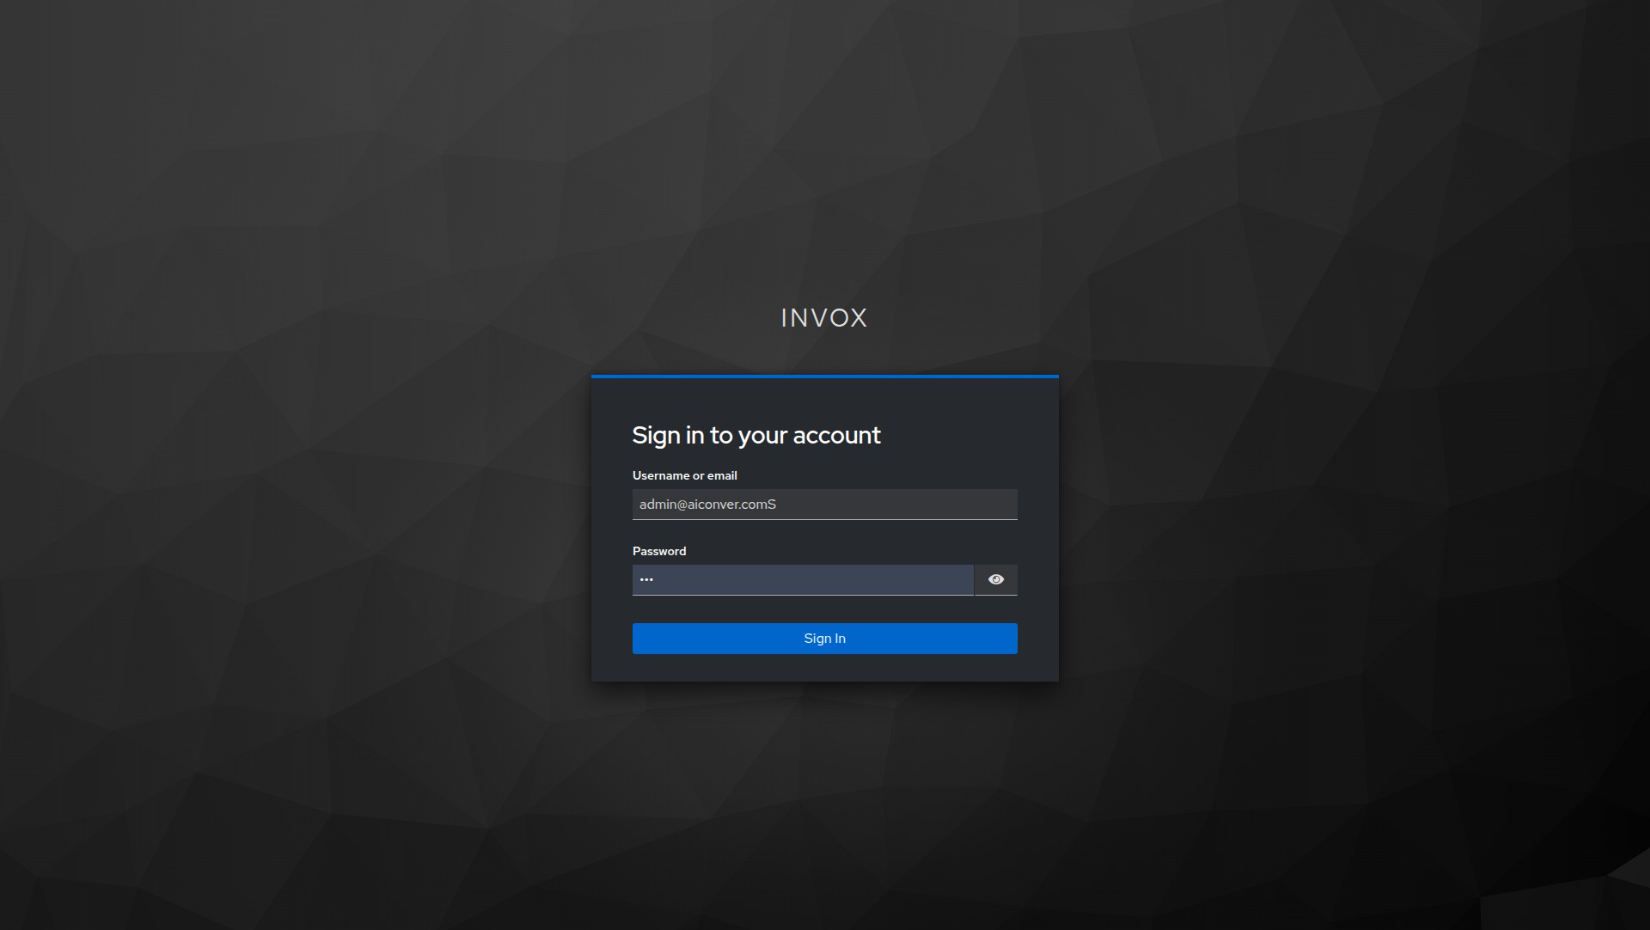
\includegraphics[width=1.0\linewidth]{images/login_interface.png}
  \caption{INVOX authentication interface with Keycloak integration}
  \label{fig:login-interface}
\end{figure}

\subsection{Template Filling Interface}
\label{subsec:ui-template-filling}

\begin{figure}[H]
  \centering
  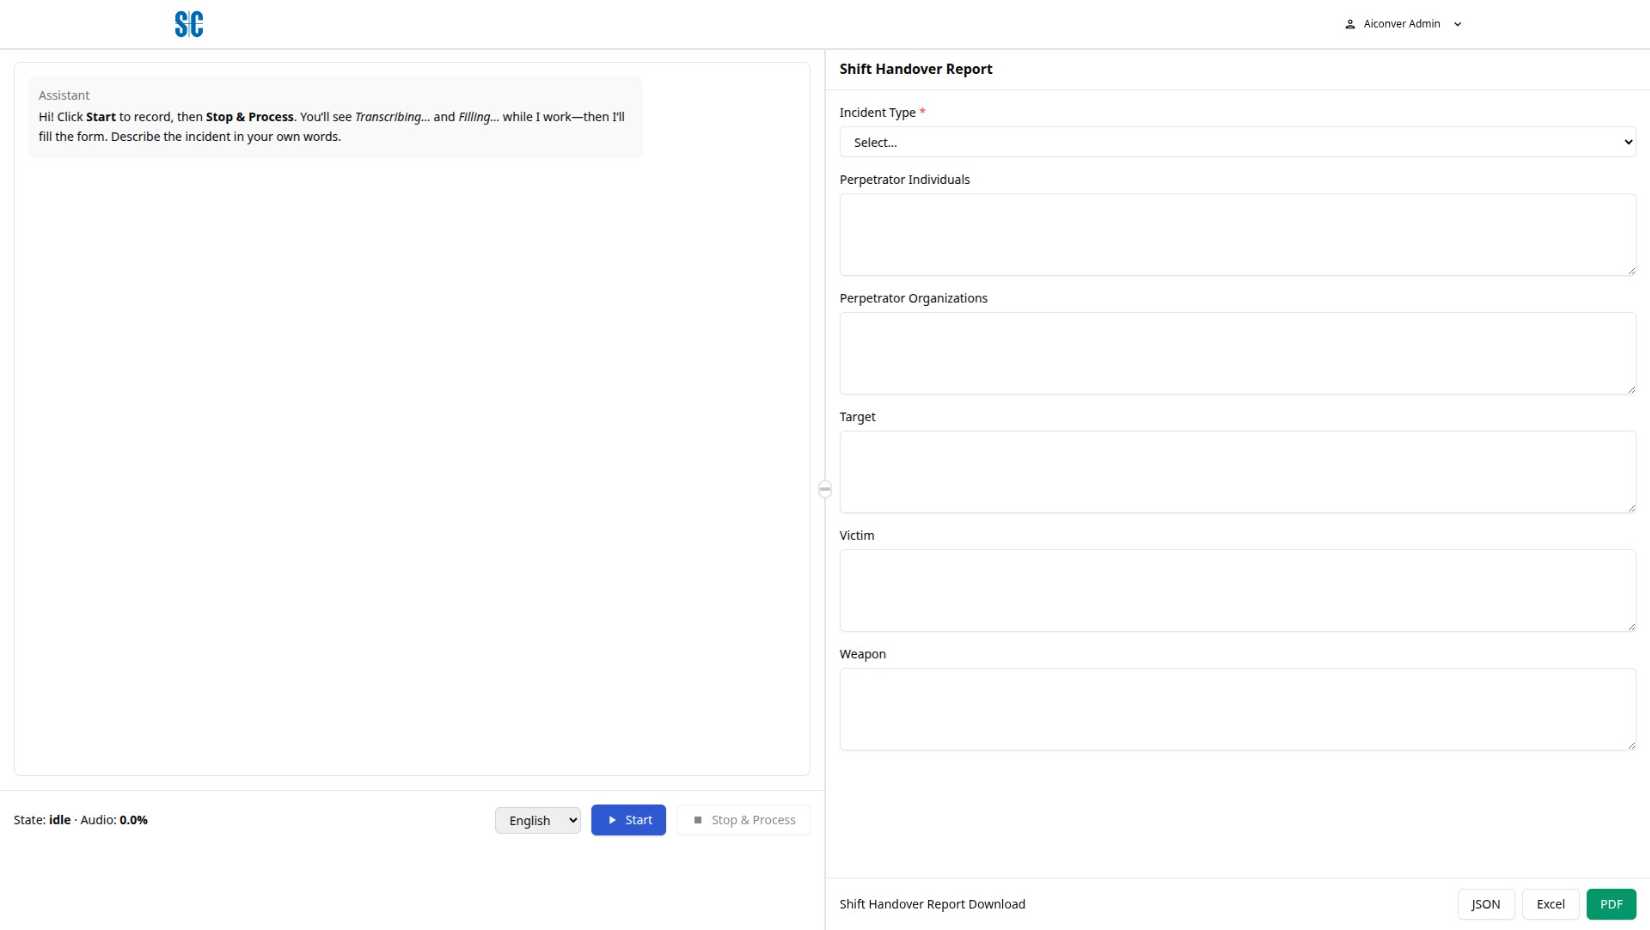
\includegraphics[width=1.0\linewidth]{images/template_interface.png}
  \caption{Template filling interface with voice input (bottom-left), structured form (right), and interactive chat panel}
  \label{fig:template-interface}
\end{figure}

The interface consists of three main components (Figure~\ref{fig:template-interface}): the audio recording panel at the bottom-left, the structured template form on the right, and an interactive chat panel for clarifications.

\subsubsection{Audio Recording Panel}

The recording panel provides a "Start" button to initiate audio capture. During recording, the button changes to "Stop \& Process." When clicked, the system transcribes the audio and extracts template values using the selected strategy. A strategy selector menu allows users to choose between S1, S2, S3, or S4 before processing, enabling them to balance speed versus accuracy based on the template's importance.

\subsubsection{Structured Template Form}

The right side displays the template form with fields organized by category (Incident Type, Perpetrator Information, Target, Victim, Weapon). As the system processes audio input, fields are automatically populated based on the extraction results. Each field type renders appropriately: dropdowns for enumerated values, text areas for descriptions, and specialized inputs for dates and numbers. Fields populated by AI extraction are marked with confidence indicators, with low-confidence fields highlighted to direct user attention.

Users can directly edit any field value, lock fields to prevent overwriting during subsequent recordings, and review the source of each value (AI-extracted versus manually entered). The form validates inputs against schema constraints before allowing submission.

\subsubsection{Interactive Chat Panel}

The chat panel provides real-time feedback during template filling. When the system identifies missing required fields, conflicting information, or ambiguous extractions, it posts messages requesting clarification. For example, if the perpetrator field contains uncertain information, the chat prompts the user to provide more specific details. This interactive guidance reduces iteration cycles by identifying issues immediately rather than after submission.

\subsection{Template Export}

Once users complete template review, the interface provides export options in JSON, Excel, and PDF formats through a download button group. All templates are automatically persisted to PostgreSQL upon processing, ensuring data preservation regardless of export actions.

Having established the complete implementation of the Invox system—from backend agent architecture to frontend user interface—the next chapter evaluates this implementation empirically. Chapter~\ref{chap:evaluation} applies the system to the MUC-4 benchmark and measures its performance against the six requirements (R1–R6) established in Chapter~\ref{chap:requirements}. The evaluation compares the four architectural strategies quantitatively, examining their trade-offs in accuracy, cost, latency, and user satisfaction.